\documentclass[12pt]{article}
\usepackage{amsmath}
\usepackage{amssymb}
\usepackage{graphicx}
\usepackage[margin=1in]{geometry}
\newcommand{\del}{\nabla}
\begin{document}

\title{Psych209 Final Project}
\author{Howon Lee}
\maketitle
\section*{Abstract}
%%% let's have the abstract last
\section*{Introduction}
\subsection*{Motivation}

We wish to use an alternative approach to add non-determinism to the constraint satisfaction problem in a PDP system, which would not be a Boltzmann machine with conventional simulated annealing.

An alternative optimization algorithm called $\tau$-extremal optimization($\tau$-EO) is used to update a constraint-satisfaction framework to escape local minima in short amounts of time. It, like simulated annealing, is inspired by condensed matter physics, but in this case, by a condensed matter model of evolution.

The update rule for Boltzmann machines in the general, non-restricted case is very powerful but not usable in practice. This is in part because of the enormous time needed to approach the network's equilibrium distribution. Therefore, other ways of avoiding local maxima and introducing nondeterminism in constraint satisfaction, besides simulated annealing of Boltzmann machines, might be of interest. Simulated annealing also has the disadvantage that it must be given an annealing schedule to work effectively, the proper tuning of which is extremely hard and problem-specific. Another source of interest is the possible exploration of the semantics of alternative ways to introduce nondeterminism into the constraint satisfaction framework in order to avoid the problem of local optima.

\subsection*{Literature Review}
%%% cite: extremal optimization, genetic algorithms
Extremal optimization, in general, is inspired by models of co-evolution. This is as opposed to genetic algorithms and evolutionary algorithms, which are inspired by evolution at a lower level of abstraction(per gene, not per species).

%%% cite: bak-sneppen, gould
To be specific, there exists a model of evolution called the Bak-Sneppen model, designed to bring about the time dynamics and other qualitative phenomena of evolution in the simplest method possible. It is a self-organized criticality model, which means that it has its attractor in a phase transition state. It is a one-dimensional lattice model which models nothing about each species except its fitness and the structure of its relations with other species. $N$ species are considered as nodes on a graph which is a one-dimensional lattice (a ring), and each species has a fitness, denoted by a single scalar $\lambda$. At each discrete time step, the least fit species is replaced, and both of its neighbors replaced with it, with new species identical to the old ones except for the fitnesses, which are random. Notably, this selection organizes a fitness threshhold, below which species do not survive because they are always the least fit.

%cite shalizi
It should be noted as important that there is not necessarily any biological reality to the model, and that it should be considered as a physical condensed-matter model.

\begin{figure}
  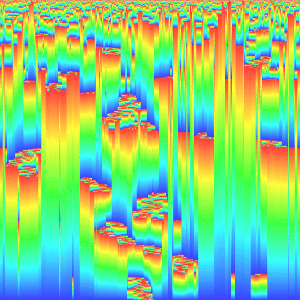
\includegraphics{bak_sneppen}
  %%% let's have a nice caption telling us stuff, citing the stuff.
\end{figure}

%%% cite Bak and Chialvo
One avenue of exploration was the adaptive extremal dynamics architecture promulgated by Bak and Chialvo as an alternative to conventional connectionist feedforward backpropagation neural nets. The topology of their alternative neural net looks much like a feedforward net, but instead of every unit forwarding its activation to the next layer, only the unit with the highest activation does so, except at the input-hidden layer.

Learning is done extremally also, in that if a wrong prediction is made, every weight going back to the input layer which was activated is punished. If a correct prediction is made, nothing is done except that the weights involved are added to a "previously made a correct prediction" list, which means that those weights are punished much less if they make a wrong prediction afterwards.

%%% cite tabu search
Bak and Chialvo note that it is very easy to make very deep nets with this architecture, since there no problem with vanishing gradients or large computations, since there are no gradients. However, this is not as useful as one might think. This is because the units end up becoming conjunctive units, bound together loosely by the effect of the "made a correct prediction list" (similar to the opposite of the Tabu list in Tabu search). This means that many thousands of units are needed to do a simple parity task, and the classification ability on naturalistic tasks like MNIST are not comparable to even linear predictors, as shown on figure \ref{fig:baknet_res}.

\begin{figure}
  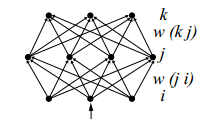
\includegraphics{bak_chialvo_net_topology}
  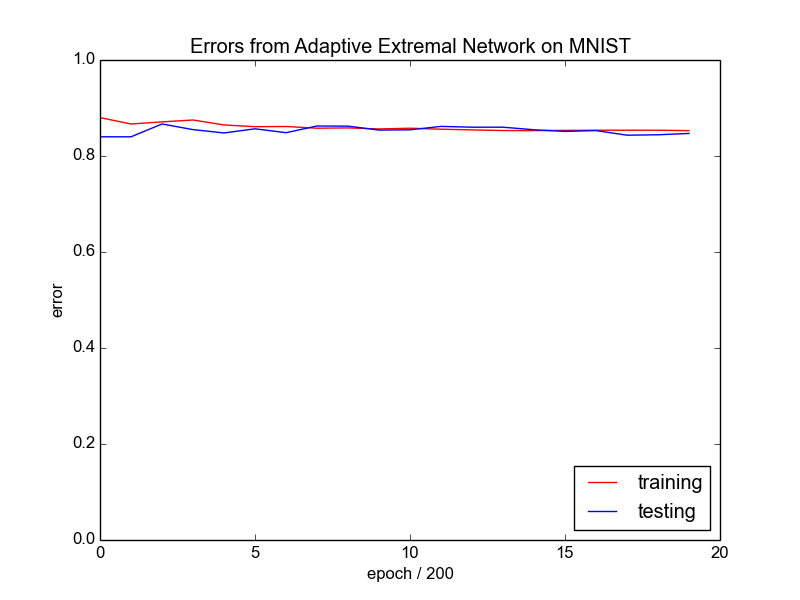
\includegraphics{bak_plot}
  \label{fig:baknet_res}
  %%% caption
\end{figure}

%%% cite Boetticher
The model creates punctuated equilibrium because as the smallest fitness increases, it becomes more likely that the next smallest fitness is adjacent to the previous smallest fitness, and therefore the events become correlated, causing "avalanches". This behavior, if one considers the nodes in the graph to be variables in a problem instead of species, was noted to be desirable in optimization problems by Boettcher and Percus, and used as the basis of extremal optimization.

Extremal optimization can be described succinctly as iteratively identifying the worst performing variable (according to the variable's fitness, which the implementer must define) in a given solution and replacing them with a new component or swapping them out with another component. Since this is trivially subject to local optima(in fact, it is just a local search), this paper will mainly deal with a variant, $\tau$-extremal optimization, which solves this problem. It does so by ordering the local fitnesses, high to low, and choosing the $k$-ranked one, where

$$P(k) = Ck^{-\tau}$$

%%% cite the analytic claim that there's an optimum value of tau.
Where $C$ is a normalizing constant and $\tau$ is the one parameter. There is a claim by Boettcher et al that there is an analytically optimal value of $\tau$ for search time, which is $\tau = 1 + \frac{1}{\ln n}$, where $n$ is the number of variables.%%% by who??

%% cite the well-defined mean shit
The reason why the $P(k)$ is the way it is is because it gives an important advantage to the search pattern of $\tau$-extremal optimization: where other search algorithms are local or global, there is no well-defined scale to its search, because the $P(k)$ is a scale-free distribution, a power law which, because $\tau < 2$, does not have a well-defined mean or variance.

%%% cite hamming cliff
This solves an important problem called the \emph{Hamming cliff} in other evolution-inspired algorithms, where very many variables are coupled in a representation, such as in a conventional binary code, where the gap between 511 (0111111111) and 512 (1000000000) needs 10 coincident mutations. What would happen in the $\tau$-extremal optimization would be that the search would eventually perversely flip the first bit, and then proceed to quickly create an avalanche where it would flip all the other bits in the representation. Also because of this property, there does not need to be anything analogous to an annealing schedule for $\tau$-extremal optimization, where a more global search transforms into a more local search.

%%% cite TSP, graph cuts, ising models, hopfield net
The previous applications of EO and $\tau$-EO include the travelling salesman problem, graph cuts and Ising model spin glass optimization. It is the last of these that seems most important for us, because of the close connection between the Hopfield net and the Ising model, and in turn the Hopfield net and the constraint satisfaction networks that exist, including the Boltzmann machine, which can be construed as a probabilistic Hopfield net.

\begin{figure}
  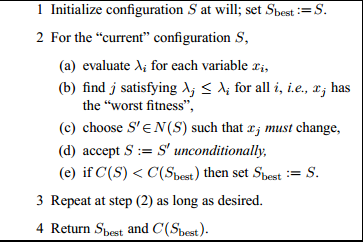
\includegraphics{eo_alg} %%%%% get a better pic
  \caption{extremal optimization algorithm}
\end{figure}

\section{Methods}

%%% cite schema network
Because of the problem of long simulation times of the Boltzmann machine and of the close relation of the Boltzmann machine to the Ising models which had already been simulated in the literature, a constraint satisfaction network was made which would have non-determinimism introduced to it by using the $\tau$-EO algorithm, just as a Boltzmann machine can be construed as a schema network with non-determinism introduced into it in another way.

%%% cite boettcher et al for the optimum of tau
In order to do this, we needed to choose a $\tau$ and to determine the fitness function. Both are fairly obvious: we chose the claimed analytic optimum from Boetcher et al and we chose the already existing goodness function from the PDP version of the schema network.

%%% cite the Boettcher thing with a heap
We want a feasible measurement of speed, which would be somewhat comparable between algorithms. However, speed in computation is complicated to measure honestly and not really germane to what is the real problem here, which is local versus global search of the problem space. For example, Boettcher et al suggest maintaining a heap in order to draw the $k$th ranked member of the local fitnesses, which is probably a sensible suggestion in their apparatus, but a whole sort of a Numpy array is actually an order of magnitude faster than the heap popping and pushing operator in Python, because it's implemented as a Python native function. And vectorization in Numpy gives two or three order-of-magnitude differences in wall-clock execution time as well. Therefore, we decided that the proper measure of execution time should actually be the number of iterations of the algorithm before converging to one of the global minima, not wall-clock time or clock-cycle time.

%%% picture of the necker cube
% did we cite frigging pdp yet? we should, really, this is a thing
Therefore, noting those problems, we chose the simplest problem possible which could test whether the $\tau$-extremal optimization was better in some way than simulated annealing or not, which is the Necker Cube constraint satisfaction problem from the PDP book. Each vertext of the Necker Cube has two units each, which represent the two interpretations of the cube, with a local minimum at the state where four units making up one face are activated in one interpretation, and the other four units making up the other face on the other interpretation are activated. This, as the PDP book mentions, is one of the sipmlest possible constraint satisfaction problems with a local optimum, which can test the claim that the $\tau$-extremal optimization gets out of local optima well.

%%% cite the Hard Parts paper
Another consideration for the measurement of speed is that there are very many initial states of activation which are trivial to turn into a global optima, but there's no really good enumeration of initial states of activation which tend to turn into local optima. Indeed, if we had one, the constraint satisfaction problem would be a great deal easier! Therefore, an honest measurement of speed would explore \emph{the entire state space} of the initial activations, or at least a representative sample of it. Since we don't necessarily know how to get a representative sample, we explore the entire initial activation state space. This was a large part of the impetus to focus on a toy problem. This was borne out in the skewed distribution of top number of iterations before convergence to a global optima.

% cite rbm
In addition, we had a preliminary investigation into trying to use the $\tau$-extremal optimization in a \emph{learning} task. Because we were investigating learning only, we decided to use a more commonly used constraint satisfier, the restricted Boltzmann machine, and then to use the more commonly used contrastive divergence to estimate the equilibrium distribution. The \emph{gradients}, not the energies, in this case were treated as the fitnesses, making this algorithm a sort of adaptive line search.

%cite the scikit-learn paper
We used, for the RBM task, a digit dataset from scikit-learn, which has 1797 samples in 10 classes. We used this instead of the more standard MNIST because it has only 64 dimensions, and it was pre-whitened and normalized.
%%% how many hiddens? what's the "learning rate"? other parameters used?
%%%%%%%%%%%%%%%%%%%%%%%%%%%%%%%%%%%%%%%%%%%%%%%%%%
%%%%%%%%%%%%%%%%%%%%%%%%%%%%%%%%%%%%%%%%%%%%%%%%%%
%%%%%%%%%%%%%%%%%%%%%%%%%%%%%%%%%%%%%%%%%%%%%%%%%%

\section{Results and Analysis}
%%% this is thin
First, the results on the RBM. We did not see the large scale-free jumps that we experienced in the Ising model and expected in the RBM. This is because the gradients with respect to the weights, which we were using as the fitness values, were local but didn't affect their neighbors in a strong way, unlike the energy calculations in the constraint satisfaction model. This ends up being essential to the punctuated-equilibrium behavior of the model.

\begin{figure}
  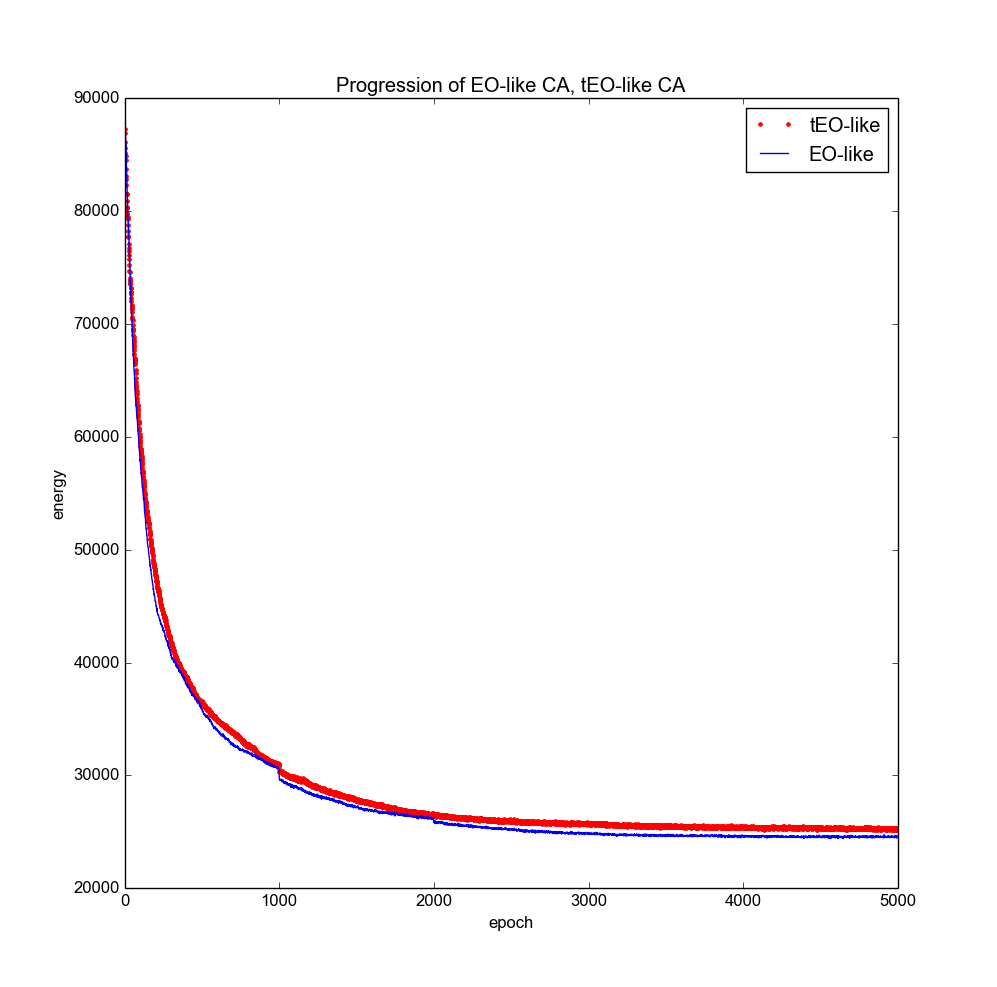
\includegraphics{eo_rbm_unzoomed}
  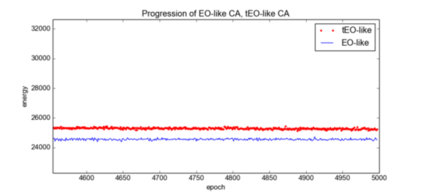
\includegraphics{eo_rbm_zoomed}
\end{figure}

The results on the $\tau$-EO necker cube task were, however, as expected. Figure \ref{fig:speed} is a histogram of the iteration numbers of each of the $2^16$ possible states before converging on a global optimum of the Necker cube task, with simulated annealing, simulated annealing with an annealing schedule, and the $\tau$-extremal optimization. Note the log-log scale.

\begin{figure}
  \label{fig:speed}
  %%%%% spiffy speed figure
  %%\includegraphics{spiffy speed thing}
\end{figure}

\begin{figure}
  \label{fig:slow_progess}
  %%\includegraphics{spiffy slow progress 1 eo}
  %%\includegraphics{spiffy slow progress 2 sa}
  \caption{Slow progress: white is positive activation}
\end{figure}
\begin{figure}
  \label{fig:fast_progess}
  %%\includegraphics{spiffy fast progress 1 eo}
  %%\includegraphics{spiffy fast progress 2 sa}
  \caption{Fast progress: white is positive activation}
\end{figure}

Note that there is a longer tail in the histogram for the simulated annealing with an annealing schedule. This is because in those cases, the simulated annealing is stuck in a local optima, and is also at a low temperature, meaning that they cannot escape this local optima. This also happens in a lesser way in the simulated annealing with constant temperature.

The majority of the time, $\tau$-extremal optimization is local search. Therefore, when it is possible to get to the global optimum by local search, it does so very quickly, as can be seen in \ref{fig:fast_progress}. An example of where $\tau$-extremal optimization goes wrong is in \ref{fig:slow_progress}, but this shows the capability that $\tau$-extremal optimization to move large distances in the activation space, by making a hugely unlikely step and then semi-locally searching from there. This is as opposed to what simulated annealing does when it degenerates, which is to get stuck in the local minima, just with the \emph{possibility} of getting out. Because at each step a move is made in $\tau$-extremal optimization, this cannot happen.

\section{Discussion}
We attempted to use $\tau$-extremal optimization in order to update a constraint satisfaction network, and compared it to the performance of simulated annealing on a Boltzmann machine on the same toy constraint satisfaction problem. As the histogram of iteration numbers shows, there was a significant gain.

%%% cite Boettcher for the disequilibrium stuff
%%% cite boettcher's heuristic about the number of iterations
An important feature of the algorithm is that it works in disequilibrium. That is, it runs the same whether it's early in the search or late in the search. Unlike simulated annealing with an annealing schedule, which doesn't work as an online algorithm, or an algorithm which can be given its input piece by piece, that there is nothing preventing $\tau$-extremal optimization from being used online. This property is of a piece with the scale-free search mentioned above. One important drawback to this is that for real problems the number of iterations needs to be determined via heuristic.

Because this project attempted to completely explore an entire state space of a problem, it was not feasible to explore a non-toy problem: that is, a problem where it's not possible to explore the entire state space, and therefore other measures of speech must be checked. It remains to be seen if this speed can be replicated in a larger problem domain with different local optima.

%% cite the chialvo paper, small world net review, modelling review
Another interesting direction would be to try to explore scale-freeness in the connectivity of the graph. Chialvo et al claim that the functional connectivity of the brain has a scale-free network character. The functional graph they create is a small world net, with a power law distribution of degree rank and a bevy of other features. This is exciting, since there is a vast literature on simulating, modelling and even fitting these graphs, and this might be of interest to connectionist modelling.

\begin{thebibliography}[99]
    Citations:   use apa
\end{thebibliography}

\end{document}

